% !TEX program = xelatex
% 基于 LLM 语义编译主动学习的多无人潜航器对海目标搜索方法
% 排版依据：《排版格式与论文书写要求》（热带生物学报/中文核心格式）
\documentclass[a4paper,UTF8,zihao=5,twocolumn]{ctexart}

% ============ 字体设置 ============
% 正文：五号宋体；英文与数字 Times New Roman
% Times New Roman 兼容字体（VM 未装 mscorefonts，TeX Gyre Termes 度量一致）
\setmainfont{TeX Gyre Termes}
\usepackage{unicode-math}
\setmathfont{TeX Gyre Termes Math}
\setCJKmainfont{Noto Serif CJK SC}           % 宋体
\setCJKsansfont{Noto Sans CJK SC}           % 黑体
\newCJKfontfamily\kaifont[AutoFakeBold=2.5]{AR PL KaitiM GB}   % 楷体
\newCJKfontfamily\fsfont[Path=/usr/share/texlive/texmf-dist/fonts/opentype/public/fandol/]{FandolFang-Regular.otf} % 仿宋
\newcommand{\kai}{\kaifont}

% ============ 页面设置：A4，双栏 ============
\usepackage[a4paper,top=2.5cm,bottom=2.5cm,left=1.8cm,right=1.8cm,columnsep=0.8cm]{geometry}
\usepackage{amsmath}
\usepackage{graphicx}
\graphicspath{{../experiments/figures/}{./}}
\usepackage{booktabs}
\usepackage{multirow}
\usepackage{caption}
\usepackage{subcaption}
\usepackage{float}
\usepackage{enumitem}
\usepackage{url}
\usepackage{xcolor}
\usepackage{setspace}

% 单倍行距；页码页脚居中，无页眉
\pagestyle{plain}
\linespread{1.05}
\setlength{\parindent}{2em}

% ============ 标题层级字体 ============
% 一级标题：小四黑体；二级：五号黑体；三级：五号楷体加粗
\ctexset{
  section = {
    format = \zihao{-4}\sffamily\bfseries,
    name = {,},
    number = \arabic{section},
    aftername = \hspace{0.5em},
    beforeskip = 1.0ex plus .2ex,
    afterskip = 1.0ex plus .2ex,
  },
  subsection = {
    format = \zihao{5}\sffamily\bfseries,
    number = \arabic{section}.\arabic{subsection},
    aftername = \hspace{0.5em},
    beforeskip = 0.8ex,
    afterskip = 0.8ex,
  },
  subsubsection = {
    format = \zihao{5}\kai\bfseries,
    number = \arabic{section}.\arabic{subsection}.\arabic{subsubsection},
    aftername = \hspace{0.5em},
    beforeskip = 0.6ex,
    afterskip = 0.6ex,
  }
}

% 图表题：小五黑体居中；编号“图 1”“表 1”
\captionsetup[figure]{font={small,sf},labelfont={sf},labelsep=quad,position=below,skip=4pt}
\captionsetup[table]{font={small,sf},labelfont={sf},labelsep=quad,position=above,skip=4pt}
\captionsetup{size=small}
\renewcommand{\figurename}{图}
\renewcommand{\tablename}{表}

% 公式编号按节连续
\numberwithin{equation}{section}

\title{}
\author{}
\date{}

% Auto-generated from experiments/results/metrics.csv — do not edit.
\newcommand{\callSfull}{80$\pm$28}
\newcommand{\callLfull}{10000$\pm$0}
\newcommand{\callRfull}{12900$\pm$1449}
\newcommand{\callS}{71}
\newcommand{\callL}{10000}
\newcommand{\callR}{12500}
\newcommand{\gainS}{99.3}
\newcommand{\ratio}{0.7}
\newcommand{\callNP}{104}
\newcommand{\pestNP}{0.0448}
\newcommand{\errNP}{19.4}
\newcommand{\callNPfull}{120$\pm$64}
\newcommand{\callNI}{66}
\newcommand{\pestNI}{0.0411}
\newcommand{\errNI}{27.2}
\newcommand{\callNIfull}{74$\pm$29}
\newcommand{\callNE}{71}
\newcommand{\pestNE}{0.0440}
\newcommand{\errNE}{30.9}
\newcommand{\callNEfull}{76$\pm$30}
\newcommand{\pestL}{0.0531}
\newcommand{\errL}{2.1}
\newcommand{\pestR}{0.0538}
\newcommand{\errR}{1.8}
\newcommand{\pestS}{0.0430}
\newcommand{\errSfull}{31.2$\pm$17.0}
\newcommand{\errS}{31.2}
\newcommand{\iouS}{0.333}
\newcommand{\callM}{98}
\newcommand{\callLM}{10000}
\newcommand{\callRM}{13500}
\newcommand{\callMfull}{106$\pm$58}
\newcommand{\pestM}{0.0430}
\newcommand{\errMfull}{33.6$\pm$23.7}
\newcommand{\iouM}{0.321}
\newcommand{\callNPmfull}{316$\pm$271}
\newcommand{\pestNPm}{0.0450}
\newcommand{\errNPm}{33.2}
\newcommand{\iouNPm}{0.235}
\newcommand{\callNPm}{252}
\newcommand{\callNImfull}{97$\pm$33}
\newcommand{\pestNIm}{0.0434}
\newcommand{\errNIm}{32.1}
\newcommand{\iouNIm}{0.270}
\newcommand{\callNIm}{101}
\newcommand{\callNEmfull}{134$\pm$108}
\newcommand{\pestNEm}{0.0412}
\newcommand{\errNEm}{35.1}
\newcommand{\iouNEm}{0.300}
\newcommand{\callNEm}{104}
\newcommand{\errM}{33.6}
\newcommand{\errLm}{5.9}
\newcommand{\errRm}{2.1}
\newcommand{\pestLm}{0.0508}
\newcommand{\pestRm}{0.0539}
\newcommand{\pctNP}{46}
\newcommand{\difNI}{-7\%}
\newcommand{\pctErrM}{4}
\newcommand{\pctErrMi}{1.5}
\newcommand{\pctNIm}{3}
\newcommand{\pctNPm}{156}
\newcommand{\pctNEm}{6}
\newcommand{\callSSfull}{76$\pm$43}
\newcommand{\pestSS}{0.0466}
\newcommand{\errSS}{16.8}
\newcommand{\iouSS}{0.366}
\newcommand{\callSS}{62}
\newcommand{\callNNfull}{119$\pm$64}
\newcommand{\pestNN}{0.0481}
\newcommand{\errNN}{19.8}
\newcommand{\iouNN}{0.399}
\newcommand{\callNN}{108}
\newcommand{\callIGfull}{111$\pm$26}
\newcommand{\pestIG}{0.0478}
\newcommand{\errIG}{12.1}
\newcommand{\iouIG}{0.857}
\newcommand{\callIG}{102}
\newcommand{\callSSmfull}{95$\pm$27}
\newcommand{\pestSSm}{0.0415}
\newcommand{\errSSm}{34.2}
\newcommand{\iouSSm}{0.327}
\newcommand{\callSSm}{86}
\newcommand{\callNNmfull}{244$\pm$183}
\newcommand{\pestNNm}{0.0438}
\newcommand{\errNNm}{24.4}
\newcommand{\iouNNm}{0.233}
\newcommand{\callNNm}{232}
\newcommand{\callIGmfull}{262$\pm$109}
\newcommand{\pestIGm}{0.0447}
\newcommand{\errIGm}{16.7}
\newcommand{\iouIGm}{0.353}
\newcommand{\callIGm}{220}
\newcommand{\pctNNm}{136}
\newcommand{\pctNNs}{53}
\newcommand{\refS}{0.0542}


\begin{document}

% ============ 题名页（跨双栏通排） ============
\twocolumn[{%
\begin{center}
  {\zihao{-2}\sffamily\bfseries 基于大语言模型语义编译主动学习的\\多无人潜航器对海目标搜索方法\par}
  \vspace{12pt}
  {\zihao{-4}\fsfont 作者一$^{1}$，作者二$^{1}$，作者三$^{2}$\par}
  \vspace{6pt}
  {\zihao{-5} （1. XX大学 XX学院，XX 000000；2. XX研究所，XX 000000）\par}
\end{center}

% 首页脚注：收稿日期、基金项目、作者简介（五号黑体标签/小五宋体内容）
\begingroup
\renewcommand{\thefootnote}{}
\footnotetext{\zihao{-5}\noindent\sffamily 收稿日期：\rmfamily 2026-10-08；
\sffamily 修回日期：\rmfamily 2026-10-08\\
\sffamily 基金项目：\rmfamily 《基金项目名称》（《项目编号》）\\
\sffamily 第一作者：\rmfamily 《姓名（出生年—），性别，学位/职称，研究方向：《研究方向》；
E-mail：《邮箱》》\\
\sffamily 通信作者：\rmfamily 《姓名，职称，研究方向；E-mail：《邮箱》》}
\endgroup

\vspace{4pt}
{\zihao{-5}\sffamily 摘\quad 要：}
{\zihao{-5}
针对多无人潜航器（UUV）对海目标搜索中全覆盖扫描效率低、文本情报与指挥意图难以注入数值搜索回路的问题，提出大语言模型（LLM）语义编译主动学习搜索方法。以深度神经网络在线构建目标存在信念图并逼近置信边界，沿边界双侧主动生成确认与排除探测任务；LLM 将情报通报编译为目标存在先验以引导初始布点，将指挥意图编译为有界采集策略参数，实现语义信息到数值控制量的合法化注入，并搭建多 UUV 搜索仿真系统验证。实验表明：在 $10^4$ 格海域内以 $\callS$ 次探测达到全覆盖扫描（$\callL$ 次）的同等判定置信度，探测成本降低 $\gainS$\%；消融实验表明先验编译接口贡献了主要成本收益，意图闭环编译在不显著增加成本的前提下提供了随态势自适应的可审计调节能力。该方法为情报驱动的自主对海搜索提供了可量化完备度判据与可解释决策链路。
\par}
\vspace{4pt}
{\zihao{-5}\sffamily 关键词：}{\zihao{-5} 对海目标搜索；主动学习；大语言模型；深度神经网络代理模型；多无人潜航器\par}
\vspace{2pt}
{\zihao{-5}\sffamily 中图分类号：}{\zihao{-5} TP391.9；TP242.6}\hfill
{\zihao{-5}\sffamily 文献标志码：}{\zihao{-5} A}\hfill
{\zihao{-5}\sffamily 文章编号：}{\zihao{-5} 1674-xxxx(2026)xx-xxxx-xx\par}
\vspace{10pt}
}]

% ============ 引言 ============
\section*{\zihao{-4}\sffamily\bfseries 引\quad 言}
\addcontentsline{toc}{section}{引言}

海洋目标搜索是反潜作战、水下搜救与海洋维权中的基础任务。多无人潜航器（uncrewed underwater vehicle, UUV）凭借隐蔽性好、续航长、可集群作业等优势，成为大范围海域搜索的重要平台\cite{ref1,ref2,ref19,ref20}。然而，水下目标具有信号弱、机动性强、先验信息稀疏等特点，传统平行往复式（lawnmower）几何覆盖搜索对探测资源的需求随海域面积线性增长，在目标高速机动场景下尤为低效。

现有搜索规划方法大体可分为三类：其一为几何覆盖方法\cite{ref3,ref4}，通过平行往复路径、螺旋路径等对责任海区进行无遗漏扫掠，工程可靠但缺乏对目标信息的利用；其二为信息论方法\cite{ref5,ref6,ref18,ref23}，以目标概率图（probability map）为状态，按信息增益或熵减最大选择探测位置，资源效率更高，但概率图难以融合文本形式的情报与指挥意图；其三为基于学习的规划方法\cite{ref7,ref8}，数据驱动的策略训练成本高，且在稀疏观测下泛化能力受限。三类方法的共同局限在于：搜索回路只能接受结构化数值输入，实际任务中大量以自然语言形式存在的情报通报、条令知识与指挥员意图无法进入决策回路。

主动学习代理模型为上述问题提供了新的思路\cite{ref14,ref15,ref16,ref17}。结构可靠性分析领域，翟东升等\cite{ref9}提出基于主动学习深度神经网络的结构可靠性分析方法（AL-DNN）：以蒙特卡洛样本为候选集，用深度神经网络逼近极限状态面，主动选取临近边界的样本调用真实模型，以很少的函数调用次数高精度识别安全/失效分界。该框架与对海搜索存在天然映射：探测动作对应昂贵函数调用，目标“可能存在/可以排除”的置信边界对应极限状态面，目标存在域占比对应失效概率。然而，将 AL-DNN 迁移至对海搜索需解决两个问题：其一，原文初始化布点为零信息均匀铺开，无法利用文本情报提供的先验线索；其二，探索/利用节奏由人工预设的超参数控制，缺乏随态势与指挥意图自适应调整的能力。

近年来大语言模型（large language model, LLM）在语义理解与推理上展现出突出能力\cite{ref10,ref11,ref24}，已在机器人任务规划\cite{ref12,ref13}等场景中用于将自然语言转化为结构化决策。受此启发，本文不令 LLM 直接生成航迹或动作，而是将其定位为\textbf{语义编译器}：把文本情报编译为数值先验、把指挥意图编译为有界策略参数，注入主动学习搜索回路，探测决策本身仍由确定性算法完成，从而兼顾 LLM 的语义能力与算法的可靠可控。

本文贡献有二：（1）提出 LLM 语义编译主动学习机制，给出“文本情报$\to$目标先验”与“指挥意图+态势$\to$有界采集参数”两个编译接口的形式化定义与输出约束，并以先验加权初始布点替代均匀布点；（2）搭建了端到端 LLM 赋能的多 UUV 对海目标搜索仿真系统，实现信念图推理、双侧任务生成、多 UUV分配、冲突消解与搜索完备度判据的完整闭环，并通过对比与消融实验验证方法有效性。

本文组织结构如下：第 1 节给出问题建模与信念图代理模型；第 2 节阐述语义编译机制与主动学习搜索方法；第 3 节给出算例研究；第 4 节总结并展望。

% ============ 1 相关理论 ============
\section{相关理论}

\subsection{对海目标搜索问题建模}

将责任海域 $D\subset\mathbb{R}^2$ 离散化为均匀网格，得到 $N$ 个候选探测点 $S=\{\symbf{x}_i\}_{i=1}^{N}$。每个候选点关联一个隐变量 $y(\symbf{x})$，表示该点处于目标存在域的程度：目标存在域内 $y>0$，其余区域 $y<0$，分界面 $y=0$ 称为\textbf{置信边界}。引入隐目标函数 $G(\symbf{x})$（类比结构可靠性分析中的极限状态函数）：对 $\symbf{x}$ 进行一次真实探测（UUV 抵近+声呐作业）可观测 $G(\symbf{x})$ 的符号与量值，但每次探测消耗燃料、时间并带来暴露风险，属昂贵调用，探测代价以调用次数度量。

定义海域目标存在域占比（area-of-presence ratio）
\begin{equation}
  P_s=\mathbb{P}\bigl(G(\symbf{x})>0\bigr)=\int_{D}\mathbb{I}\bigl(G(\symbf{x})>0\bigr)\,\mathrm{d}\symbf{x}/|D|,
  \label{eq:ps}
\end{equation}
其中 $\mathbb{I}(\cdot)$ 为示性函数。$P_s$ 类比结构可靠性中的失效概率 $P_f$：当 $P_s\to0$ 时可声明“目标不在该海域”，其估计精度直接度量搜索完备度。搜索任务的目标为：以尽可能少的探测次数将 $P_s$ 估计至给定置信精度，并使剩余判定不确定性集中于置信边界邻域。

对蒙特卡洛估计，取 $N_{MC}$ 个均匀采样点 $\{\symbf{x}_j^{MC}\}$，其估计量为
\begin{equation}
  \hat{P}_s=\frac{1}{N_{MC}}\sum_{j=1}^{N_{MC}}\mathbb{I}\bigl(\hat{G}(\symbf{x}_j^{MC})>0\bigr),
  \label{eq:mcs}
\end{equation}
其中 $\hat{G}$ 为代理模型预测。估计的变异系数为
\begin{equation}
  \mathrm{cov}(\hat P_s)=\sqrt{\frac{1-\hat P_s}{N_{MC}\hat P_s}},
  \label{eq:cov}
\end{equation}
由于 $N_{MC}$ 较大，代理模型侧的蒙特卡洛误差可忽略；实际计算中采用 $n_f$ 次独立重复估计的标准差与均值之比度量收敛
\begin{equation}
  \varepsilon=\frac{\sigma(\hat P_s)}{\mu(\hat P_s)},
  \label{eq:eps}
\end{equation}
当 $\varepsilon\leq\varepsilon_s$（本文取 $\varepsilon_s=0.02$）时判定收敛，输出搜索完备度声明。

\subsection{信念图代理模型}

信念图由深度神经网络 $\hat G(\symbf{x};\symbf{\theta})$ 在线逼近。输入为候选点坐标，网络含若干隐层，激活函数采用 Swish 函数
\begin{equation}
  \mathrm{Swish}(z)=z\cdot\mathrm{sigmoid}(\beta z),\quad \beta=1,
  \label{eq:swish}
\end{equation}
输出为 $\hat G$ 的标量预测。令已探测样本集（主动学习数据集）为 $\mathrm{DoE}=\{(\symbf{x}_i,G_i)\}_{i=1}^{n}$，训练损失取边界加权均方误差
\begin{equation}
  \mathcal{L}=\frac{1}{n}\sum_{i=1}^{n}w_i\bigl(\hat G(\symbf{x}_i;\symbf{\theta})-G_i\bigr)^2,\quad
  w_i=\frac{1}{|G_i|+c},
  \label{eq:loss}
\end{equation}
其中常数 $c=0.25$ 防止 $|G_i|$ 过小时权重发散。式\eqref{eq:loss}使临近置信边界的样本获得更大训练权重，直接提高边界识别精度。

参照文献\cite{ref9}的增量更新策略：每轮新增探测样本后，网络以上一轮权重 $\symbf{\theta}_{k-1}$ 为初值继续训练（权重继承），而非重新初始化，显著降低单轮训练开销并稳定收敛轨迹。

% ============ 2 方法 ============
\section{基于 LLM 语义编译的主动学习对海搜索方法}

方法总体框架如图\ref{fig:arch}所示。LLM 语义编译器将两类非结构化输入编译为数值量注入 AL-DNN 搜索回路：情报通报编译为目标存在先验分布，指挥意图编译为有界采集策略参数；回路内部为确定性算法，完成先验引导初始布点、双侧主动采样、多 UUV批量探测与收敛判定。

\begin{figure*}[!t]
  \centering
  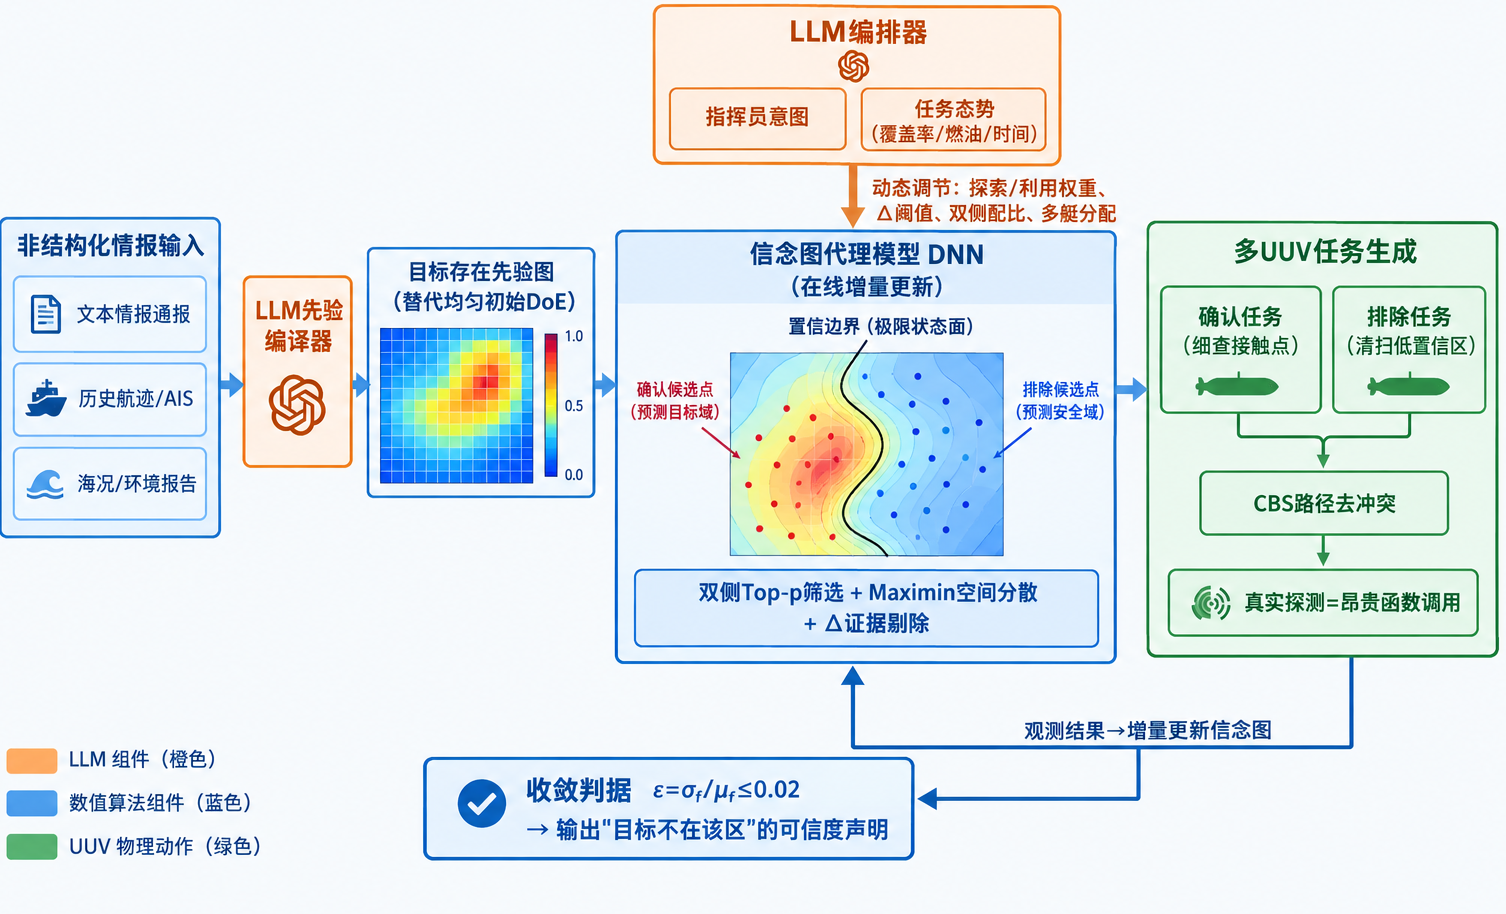
\includegraphics[width=0.95\textwidth]{fig_sys_arch.png}
  \caption{基于 LLM 语义编译的主动学习对海搜索方法总体框架}
  \label{fig:arch}
\end{figure*}

\subsection{语义编译机制}

\subsubsection{文本情报到目标先验的编译}

情报通报（海情简报、历史接触记录、第三方告警等）以自然语言描述目标可能位置、运动趋势与置信度。定义编译算子
\begin{equation}
  \mathcal{C}_I:\ \text{情报文本}\longrightarrow \pi(\symbf{x})=\sum_{m=1}^{M}\tilde w_m\,\mathcal{N}(\symbf{x};\symbf{\mu}_m,\symbf{\Sigma}_m),
  \label{eq:compile-prior}
\end{equation}
其中 $\pi(\symbf{x})$ 为归一化目标存在先验密度，由 LLM 输出的若干高斯热点分量 $(\symbf{\mu}_m,\symbf{\Sigma}_m,\tilde w_m)$ 混合而成，并附总体置信度 $c_\pi\in[0,1]$。当 $c_\pi$ 低于阈值或解析失败时，$\pi$ 退化为均匀分布，算法行为自动退化为无先验版本，保证语义信息的接入不改变方法收敛成本的最坏情形有界性（第 3.5 节对该性质进行实验验证）。

\subsubsection{指挥意图到采集策略参数的编译}

指挥意图文本与实时态势摘要（覆盖率、已探测次数、目标命中数、剩余燃料等）经编译算子
\begin{equation}
  \begin{split}
    \mathcal{C}_P:\ (\text{意图文本},\text{态势})&\longrightarrow
    \symbf{\lambda}\\[-2pt]
    &=(p_0,p_{\min},\eta,\Delta,r_d,w_e,B)
  \end{split}
  \label{eq:compile-intent}
\end{equation}
映射为主动学习策略参数向量，各参数含义与取值界见表\ref{tab:schema}。编译输出先经结构化校验，再逐项钳制到算法稳定域内
\begin{equation}
  \lambda_j^{\mathrm{eff}}=
  \begin{cases}
    \min(\lambda_j^{+},\max(\lambda_j^{-},\lambda_j^{LLM})), & \text{合法}\\
    \lambda_j^{\mathrm{def}}, & \text{解析失败/越界}
  \end{cases}
  \label{eq:clamp}
\end{equation}
其中 $\lambda_j^{-},\lambda_j^{+}$ 为表\ref{tab:schema}给出的取值界，$\lambda_j^{\mathrm{def}}$ 为默认值。LLM 不能越界改变算法语义——探测点的选取、任务的生成与收敛的判定均由确定性规则完成。该“LLM 调参、算法执行”的分工使机制具备可审计性：每次编译的输入文本、输出参数与实际生效值均被记录，形成可回溯的决策链。

编译算子以闭环方式生效：任务开始前由指挥意图与初始态势生成首版参数；搜索过程中每隔 $K_p$ 轮（本文取 $K_p=20$）将最新态势摘要（已探测次数、存在域命中数、当前 $\hat P_s$ 估计等）连同原意图重新编译，输出的有界参数自下一轮起生效。意图编译由此构成随态势演化的闭环调节，而非一次性参数整定；全部再编译调用的输入文本与输出参数均被同等记录。

\begin{table}[!t]
  \centering
  \caption{采集策略参数 Schema}
  \label{tab:schema}
  \resizebox{\columnwidth}{!}{%
  \begin{tabular}{cccc}
    \toprule
    参数 & 含义 & 取值界 & 默认值 \\
    \midrule
    $p_0$ & 初始筛选比例 & $[0.2,0.8]$ & 0.4 \\
    $p_{\min}$ & 筛选比例下限 & $[0.02,0.30]$ & 0.05 \\
    $\eta$ & 比例衰减速率 & $[0.60,0.95]$ & 0.80 \\
    $\Delta$ & 证据老化权重阈值 & $[0.02,0.30]$ & 0.10 \\
    $r_d$ & 双侧任务配比 & $[0.30,0.70]$ & 0.50 \\
    $w_e$ & 探索权重 & $[0.50,1.50]$ & 1.00 \\
    $B$ & 批量探测规模/UUV·轮 & $[2,8]$ & 4 \\
    \bottomrule
  \end{tabular}}%
\end{table}

\subsection{先验引导的初始布点}

原文献采用零信息 Maximin 布点：从候选集中反复选取距已选点最远的候选点，几何上均匀铺开。本文将目标先验引入初始主动学习数据集构建：先从 $S$ 中依密度 $\pi(\symbf{x})$ 抽取大小为 $6n_{init}$ 的候选池
\begin{equation}
  \mathcal{P}\sim\mathrm{Categorical}\bigl(6n_{init};\,\pi(\symbf{x})\bigr),
  \label{eq:pool}
\end{equation}
再在池内执行 Maximin 选取：第 $i$ 个初始探测点取为
\begin{equation}
  \symbf{x}_i^{\ast}=\arg\max_{\symbf{x}\in\mathcal{P}\setminus\mathrm{DoE}_{i-1}}\ \min_{\symbf{x}'\in\mathrm{DoE}_{i-1}}\|\symbf{x}-\symbf{x}'\|_2,
  \label{eq:maximin}
\end{equation}
其中 $\mathrm{DoE}_{i-1}$ 为已选点集。当先验集中于少数热点时，初始样本在热点区内加密、在其余区域保持稀疏覆盖，兼顾先验利用与全局可行性。

\subsection{双侧采样与多 UUV批量探测}

每轮迭代按以下步骤执行：

\textbf{（1）信念图更新。} 以当前 DoE 按式\eqref{eq:loss}增量训练 $\hat G$，并在蒙特卡洛候选集上预测 $\hat P_s$，累计 $n_f$ 轮估计后按式\eqref{eq:eps}计算收敛度。

\textbf{（2）双侧候选筛选。} 对全体候选点预测 $\hat G$。以筛选比例
\begin{equation}
  p_k=\max\bigl(p_{\min},\ p_0\cdot\eta^{k-1}\bigr)
  \label{eq:pk}
\end{equation}
自置信边界两侧分别构造候选子集
\begin{equation}
\begin{aligned}
  \mathcal{S}_k^{+}&=\mathrm{top\text{-}}p_k\bigl\{|\hat G(\symbf{x})|:\hat G(\symbf{x})>0\bigr\},\\
  \mathcal{S}_k^{-}&=\mathrm{top\text{-}}p_k\bigl\{|\hat G(\symbf{x})|:\hat G(\symbf{x})\le0\bigr\},
\end{aligned}
  \label{eq:twoside}
\end{equation}
即预测存在域侧与预测排除域侧各取 $|\hat G|$ 最小（最靠近边界）的前 $p_k$ 比例候选点，分别生成\textbf{确认任务}与\textbf{排除任务}候选集合。双侧采样使探测资源集中于判定信息量最大的边界带，而非已确知区域内部。

\textbf{（3）多 UUV批量生成。} 每轮共选取 $B$ 个探测点并指派至多艘 UUV 并行执行，确认/排除两类任务数量按配比 $r_d$ 划分
\begin{equation}
  B_{n}=\lceil r_d\,\tilde B\rceil,\quad B_{p}=\tilde B-B_{n},\quad \tilde B=B-B_{e},
  \label{eq:quota}
\end{equation}
其中 $B_n$、$B_p$ 分别为确认任务与排除任务的探测点数，$r_d$ 为确认任务占比（$r_d>0.5$ 偏确认、$<0.5$ 偏排除），$B_e$ 为保留的全局探索份额
\begin{equation}
  B_{e}=\mathrm{clip}\bigl(\mathrm{round}(0.25\,w_e B),\,1,\,\lfloor B/2\rfloor\bigr),
  \label{eq:explore}
\end{equation}
存在域尚未命中时式\eqref{eq:explore}被覆盖为 $B_e=\lfloor B/2\rfloor$，以扩大排除域探测份额，防止代理模型陷入“全域安全”假象（即代理模型将全域误判为可排除域而提前满足收敛判据的失效模式）。两侧候选子集内分别按式\eqref{eq:maximin}的 Maximin 原则选点以保证艇间分散；一侧候选不足时配额自动让渡给另一侧。各点指派至空闲 UUV 后，经基于冲突的搜索（conflict-based search）\cite{ref21}消解路径冲突、按 Dubins 运动约束\cite{ref22}生成可行航迹下发执行。

\textbf{（4）证据老化剔除。} 机动目标使历史探测结论失效。记第 $i$ 个 DoE 样本的观测龄期为
\begin{equation}
  a_i(k)=k-k_i^{\mathrm{obs}},
  \label{eq:age}
\end{equation}
其中 $k_i^{\mathrm{obs}}$ 为其观测时刻、$k$ 为当前迭代轮次。训练时对该样本施加衰减权重
\begin{equation}
  w_i^{\mathrm{age}}=e^{-a_i(k)/\tau},
  \label{eq:agew}
\end{equation}
$\tau$ 为衰减常数，陈旧证据在训练中的影响趋零；对“无目标”观测（$G_i\le0$），当
\begin{equation}
  w_i^{\mathrm{age}}<\Delta
  \label{eq:reverify}
\end{equation}
时其“已扫清空”结论失效，所在单元回归排除侧候选集合等待复验；存在域命中样本仅降权、不剔除，防止目标痕迹被错误遗忘。该机制对应文献\cite{ref9}的 $\Delta$ 剔除在时变场景下的推广。

\textbf{（5）收敛判定。} 满足 $\varepsilon\leq\varepsilon_s$、迭代数不低于下限且 $\hat P_s$ 估计未退化为零时终止搜索，输出 $\hat P_s$、置信边界与完备度声明。

\subsection{算法流程}

算法步骤归纳如下：

\textbf{步骤 1}：语义编译。LLM 将情报文本编译为先验 $\pi(\symbf{x})$，将指挥意图与初始态势编译为策略参数 $\symbf{\lambda}$，经界约束后生效。

\textbf{步骤 2}：初始布点。按第 2.2 节先验加权 Maximin 生成 $n_{init}$ 个初始探测点并执行探测，构建初始 DoE。

\textbf{步骤 3}：信念图拟合。按式\eqref{eq:loss}增量训练 $\hat G$；在 $N_{MC}$ 个蒙特卡洛样本上按式\eqref{eq:mcs}估计 $\hat P_s$。

\textbf{步骤 4}：收敛判据。累计 $n_f$ 次估计后计算 $\varepsilon$，满足式\eqref{eq:eps}判据则转步骤 7。

\textbf{步骤 5}：双侧采样与批量指派。按式\eqref{eq:pk}确定 $p_k$，边界两侧筛选候选并生成确认/排除任务；候选子集内 Maximin 批量选取并分配至各 UUV。

\textbf{步骤 6}：探测与老化。执行探测更新 DoE；样本按龄期衰减，权重低于 $\Delta$ 的“已扫清空”结论失效并回归候选集合等待复验；目标机动时同步更新隐目标场。每满 $K_p$ 轮将最新态势摘要连同指挥意图重新编译更新 $\symbf{\lambda}$。转步骤 3。

\textbf{步骤 7}：输出结果。输出 $\hat P_s$ 及其收敛度、置信边界预测与剩余高存在域，给出搜索完备度声明。

% ============ 4 案例研究 ============
\section{案例研究}

\subsection{算例设置与仿真环境}

仿真海域归一化为 $[0,1]^2$、离散为 $100\times100$ 网格（$N=10^4$ 候选点）。目标存在域由若干椭圆形高值子区叠加并截断至有限值域构成隐目标场 $G$；机动场景下存在域按固定漂移速度场逐迭代平移。探测模型：UUV 对指派点执行一次探测即返回 $G(\symbf{x})$ 观测，探测代价以调用次数 $N_{\mathrm{call}}$ 统一度量。蒙特卡洛估计规模 $N_{MC}=2\times10^4$。主要仿真参数见表\ref{tab:sim}。

除探测次数外，采用两项精度指标：相对误差
\begin{equation}
  \mathrm{err}=\frac{|\hat P_s-P_s^{\ast}|}{P_s^{\ast}}\times100\%,
  \label{eq:err}
\end{equation}
其中 $P_s^{\ast}$ 为全域逐点真值计算得到的参考值；以及预测存在域与真实存在域的边界交并比
\begin{equation}
\begin{aligned}
  \mathrm{IoU}&=\frac{|\hat\Omega^{+}\cap\Omega^{+}|}{|\hat\Omega^{+}\cup\Omega^{+}|},\\
  \Omega^{+}&=\{\symbf{x}:G(\symbf{x})>0\},\ \hat\Omega^{+}=\{\symbf{x}:\hat G(\symbf{x})>0\}.
\end{aligned}
  \label{eq:iou}
\end{equation}

需说明两项指标的口径差异：参考值 $P_s^{\ast}$ 由连续海域上的蒙特卡洛积分给出，而各方法在 $N=10^4$ 离散网格上估计 $\hat P_s$；故全覆盖扫描即便扫满全部格点仍残存约 $2\%$ 的口径误差，属离散化估计与真值域的差异而非判定错误。

\begin{table}[!t]
  \centering
  \caption{仿真参数设置}
  \label{tab:sim}
  \resizebox{\columnwidth}{!}{%
  \begin{tabular}{ccc}
    \toprule
    参数 & 取值 & 含义 \\
    \midrule
    网格规模 $N$ & $100\times100$ & 候选探测点数 \\
    初始探测点数 $n_{init}$ & 24 & 初始 DoE 规模 \\
    蒙特卡洛样本 $N_{MC}$ & $2\times10^4$ & $\hat P_s$ 估计规模 \\
    收敛阈值 $\varepsilon_s$ & 0.02 & 式\eqref{eq:eps}判据 \\
    估计窗口 $n_f$ & 10 & 收敛统计轮数 \\
    迭代上限 & 160 & 强制终止轮数 \\
    意图重编译周期 $K_p$ & 20 迭代 & 闭环意图更新 \\
    漂移速度 & $(0.0025,-0.002)$/迭代 & 机动目标算例 \\
    证据衰减常数 $\tau$ & 8 迭代 & 老化权重时间常数 \\
    \bottomrule
  \end{tabular}}%
\end{table}

需说明“多 UUV”的建模口径：本文以每轮批量探测规模 $B$ 抽象多艇协同（$B$ 个并行探测点对应 $B$ 艇作业），艇间动力学与航路代价未单独建模——该简化下探测次数即多艇总探测成本的度量，更精细的艇级运动建模列为后续工作。

为验证方法有效性，设计两组算例：静态目标算例检验基本收敛性能，机动目标算例检验证据老化机制。每组算例设置两类对比：基线方法（全覆盖扫描、随机采样、信息增益），以及五组消融配置——\textbf{无先验}（初始布点退化为均匀 Maximin）、\textbf{无意图}（策略参数取表\ref{tab:schema}默认值且不再更新）、\textbf{无剔除}（关闭证据老化机制）、\textbf{单侧采样}（取消确认/排除双侧划分，仅以 $|\hat G|$ 最小的单一近界候选池承载全部任务额度）、\textbf{无先验无意图}（同时移除先验与意图编排）。信息增益基线与本文方法共用代理模型与 $\varepsilon$ 停机判据，每轮贪婪选取预测存在概率最接近 $0.5$（Bernoulli 熵最大）的 $B$ 个候选点，但无语义先验、无双侧配比与证据老化——用于隔离信息论路线与本文机制的贡献差异。每一配置独立重复 10 次。鉴于探测次数呈右偏长尾分布且个别轮次会耗尽迭代上限（此类轮次单独标注“未收敛”而非计入方差放大），本文统一按 SCI 惯例报告均值$\pm$标准差、中位数与四分位距（IQR）；柱状图与折线图误差棒取中位绝对偏差（median absolute deviation, MAD，乘以 1.4826 归一化），与柱高中的中位数点估计同心，对长尾噪声稳健；全部逐次数据、统计汇总与收敛曲线数据以 Excel 数据文件随文提供。LLM 编译调用真实大模型接口完成，情报与意图文本及模型输出随数据文件一并提供。

\subsection{静态目标算例}

海域内布置三个椭圆形存在域子区（参数见表\ref{tab:sim}），真实 $P_s^\ast=\refS$。情报通报描述“两处高可能热点与两处次级可能区域”，LLM 编译得到的先验如图\ref{fig:map}(b)所示——热点分量位置与真实存在域基本重合；指挥意图“较快普查、节省燃油”被编译为中等批量、较慢衰减的策略（$p_0=0.6,B=6,\eta=0.85$）。

图\ref{fig:map}给出本方法一次典型运行的探测点分布与预测置信边界：探测点密集分布于边界两侧与先验热点区，预测边界（品红虚线）与真实存在域边界高度重合，边界交并比 IoU 达 $\iouS$。

\begin{figure*}[!t]
  \centering
  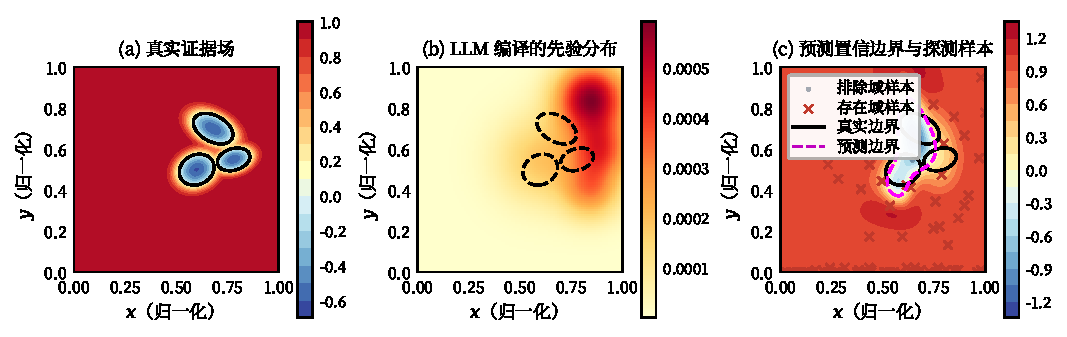
\includegraphics[width=0.98\textwidth]{fig_sampling_map.pdf}
  \caption{静态算例探测结果：(a) 真实目标场；(b) LLM 先验密度；(c) 置信边界与探测点分布}
  \label{fig:map}
\end{figure*}

图\ref{fig:conv-s}为各方法 $\hat P_s$ 随探测次数的收敛曲线（10 次重复中位数）。本方法在约 $\callS$ 次探测后收敛，全覆盖扫描与随机采样分别需要 $\callL$、$\callR$ 次；三种方法 $\hat P_s$ 终值与真值的相对误差均在 $\errS$\% 量级，判定结论一致。

\begin{figure}[!t]
  \centering
  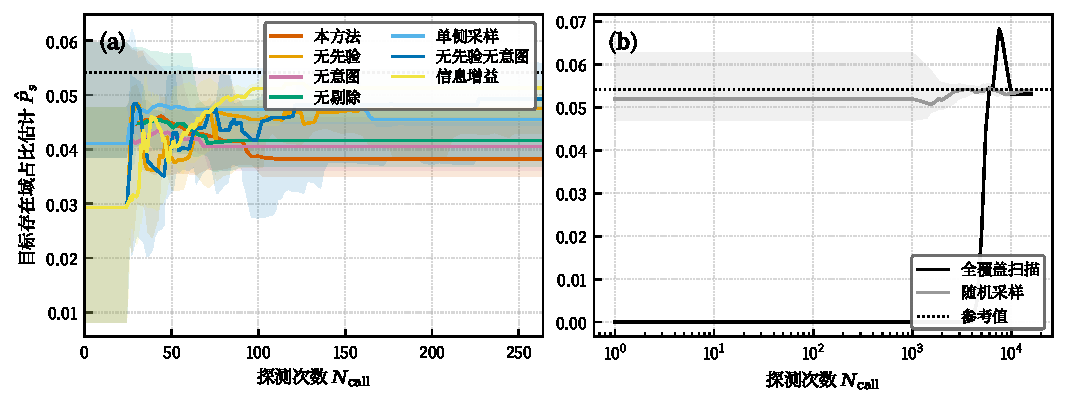
\includegraphics[width=\columnwidth]{fig_convergence_static.pdf}
  \caption{静态算例 $\hat P_s$ 收敛曲线（10 次重复中位数，阴影带为四分位距）}
  \label{fig:conv-s}
\end{figure}

\begin{table}[!t]
  \centering
  \caption{静态算例方法对比（10 次重复均值$\pm$标准差）}
  \label{tab:res-static}
  \resizebox{\columnwidth}{!}{%
  \begin{tabular}{lccc}
    \toprule
    方法 & 探测次数 & $\hat P_s$ & 相对误差/\% \\
    \midrule
    本方法 & $\callSfull$ & $\pestS$ & $\errSfull$ \\
    \quad 无先验 & $\callNPfull$ & $\pestNP$ & $\errNP$ \\
    \quad 无意图 & $\callNIfull$ & $\pestNI$ & $\errNI$ \\
    \quad 无剔除 & $\callNEfull$ & $\pestNE$ & $\errNE$ \\
    \quad 单侧采样 & $\callSSfull$ & $\pestSS$ & $\errSS$ \\
    \quad 无先验无意图 & $\callNNfull$ & $\pestNN$ & $\errNN$ \\
    信息增益 & $\callIGfull$ & $\pestIG$ & $\errIG$ \\
    全覆盖扫描 & $\callLfull$ & $\pestL$ & $\errL$ \\
    随机采样 & $\callRfull$ & $\pestR$ & $\errR$ \\
    \bottomrule
  \end{tabular}}%
\end{table}

由表\ref{tab:res-static}可见：所提方法以 $\callSfull$ 次探测收敛，约为全覆盖扫描（$\callLfull$ 次）的 $\ratio$\%，成本降低 $\gainS$\%；各主动学习配置的 $\hat P_s$ 均收敛至参考值 $\refS$ 附近（相对误差约 $\errS$\%），判定结论与全覆盖方案一致。移除语义先验后探测次数增至 $\callNP$（+$\pctNP$\%）、相对误差升至 $\errNP$\%，表明先验引导的初始布点有效压缩了早期全局探查成本；移除意图编排采用固定默认参数时探测次数反而略低（$\callNI$，$\difNI$），说明意图接口对收敛成本的独立影响在两组算例中均不显著，其价值在于闭环自适应与可审计性而非成本优势（详见第 3.4 节综合讨论）；静态场景下证据老化机制不触发，“无剔除”与本方法等价。信息增益基线探测次数中位数为 102 次，高于本方法的 71 次——其按全局熵贪婪布点，需将不确定性在全场内均匀压减方能满足 $\varepsilon$ 判据，收敛更慢；作为代价的反面，其边界 IoU 均值达 0.857，显著高于本方法的 0.333，说明信息论路线得到的是更精细的全场概率图，而本文边界聚焦采样以更低的探测成本换取够用的边界定位，二者分别适用于“精细制图”与“快速判定”两类任务需求。

\subsection{机动目标算例}

目标存在域以 $(0.0025,-0.002)$/迭代的速度场漂移。LLM 据机动通报与意图“时效优先、容忍探索”输出更激进策略（$B=8,w_e=1.5,\Delta=0.15$）。图\ref{fig:conv-m}为收敛曲线：本方法经 $\callM$ 次探测收敛，全覆盖扫描与随机采样分别需 $\callLM$、$\callRM$ 次，且后两者在漂移场景下估计偏差显著增大。

\begin{figure}[!t]
  \centering
  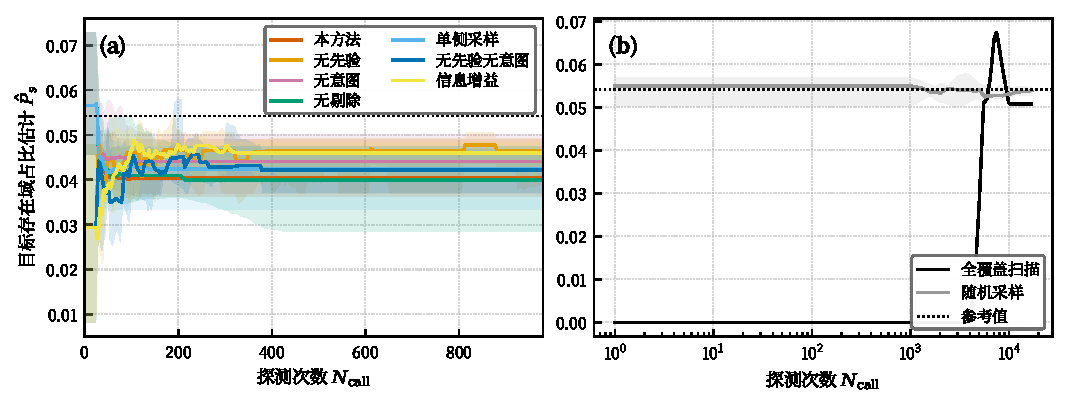
\includegraphics[width=\columnwidth]{fig_convergence_moving.pdf}
  \caption{机动算例 $\hat P_s$ 收敛曲线（10 次重复中位数，阴影带为四分位距）}
  \label{fig:conv-m}
\end{figure}

表\ref{tab:res-moving}给出机动算例方法对比。本方法以 $\callMfull$ 次探测收敛，全覆盖扫描与随机采样分别需 $\callLM$ 与 $\callRM$ 次；移除先验后探测次数增至 $\callNPmfull$（+$\pctNPm$\%），远超静态场景的影响幅度——机动场景下先验对快速锁定移动目标尤为关键；移除意图编排后探测次数基本相当（$\callNImfull$，+$\pctNIm$\%，统计不显著）——意图接口的成本效应有限，其价值在于闭环自适应与可审计性（见第 3.4 节）；移除证据老化后探测次数与本方法相当（$\callNEmfull$，+$\pctNEm$\%）、边界 IoU 基本持平（$\iouM$ 对 $\iouNEm$），其收益主要体现于边界跟踪的时效性——图\ref{fig:mmap}显示无老化时预测边界明显滞后于漂移方向。信息增益基线在机动场景下退化明显（中位数 220 次，约为本方法的 2.2 倍）：缺乏证据老化机制使陈旧观测持续干扰代理模型，全局熵布点难以跟上漂移的存在域，验证了语义编译机制相对纯信息论路线的适配优势。

\begin{table}[!t]
  \centering
  \caption{机动算例方法对比（10 次重复均值$\pm$标准差）}
  \label{tab:res-moving}
  \resizebox{\columnwidth}{!}{%
  \begin{tabular}{lcccc}
    \toprule
    方法 & 探测次数 & $\hat P_s$ & 相对误差/\% & 边界 IoU \\
    \midrule
    本方法 & $\callMfull$ & $\pestM$ & $\errMfull$ & $\iouM$ \\
    \quad 无先验 & $\callNPmfull$ & $\pestNPm$ & $\errNPm$ & $\iouNPm$ \\
    \quad 无意图 & $\callNImfull$ & $\pestNIm$ & $\errNIm$ & $\iouNIm$ \\
    \quad 无剔除 & $\callNEmfull$ & $\pestNEm$ & $\errNEm$ & $\iouNEm$ \\
    \quad 单侧采样 & $\callSSmfull$ & $\pestSSm$ & $\errSSm$ & $\iouSSm$ \\
    \quad 无先验无意图 & $\callNNmfull$ & $\pestNNm$ & $\errNNm$ & $\iouNNm$ \\
    信息增益 & $\callIGmfull$ & $\pestIGm$ & $\errIGm$ & $\iouIGm$ \\
    全覆盖扫描 & $\callLM$ & $\pestLm$ & $\errLm$ & -- \\
    随机采样 & $\callRM$ & $\pestRm$ & $\errRm$ & -- \\
    \bottomrule
  \end{tabular}}%
\end{table}

图\ref{fig:mmap}对比有/无证据老化剔除下机动算例末轮探测点分布：无剔除时陈旧观测干扰边界拟合，预测边界明显滞后于真实存在域漂移方向；启用剔除后边界紧跟真实场。

\begin{figure*}[!t]
  \centering
  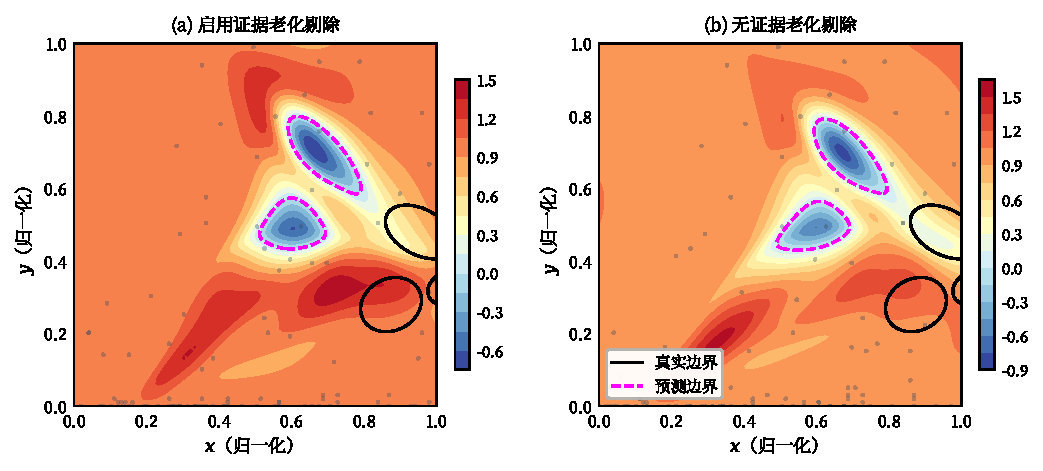
\includegraphics[width=0.92\textwidth]{fig_moving_map.pdf}
  \caption{机动算例末轮状态对比：(a) 含证据老化剔除；(b) 无剔除}
  \label{fig:mmap}
\end{figure*}

\subsection{消融实验}

综合两算例的消融结果（图\ref{fig:ablation}，表\ref{tab:res-static}、\ref{tab:res-moving}）：（1）语义先验是收益最显著的组件，移除后静态、机动场景探测次数分别增加 $\pctNP$\% 与 $\pctNPm$\%，验证"文本情报$\to$数值先验"编译接口的有效性；（2）意图编排对探测次数的独立影响不显著（静态 $\difNI$、机动 +$\pctNIm$\%，Wilcoxon 检验均不显著）——意图接口的可测量收益不在收敛成本；从重编译日志看，闭环编译使策略参数随态势演化（如收敛临近时收紧批量与探索权重），其作用是为指挥意图提供可审计的有界自适应调节通道；（3）证据老化在静态场景不触发（与本方法等价）；在机动场景移除后探测次数仅增 $\pctNEm$\%、边界 IoU 基本持平，量化收益有限，但图\ref{fig:mmap}显示无老化时预测边界明显滞后于真实存在域漂移方向——该机制主要保障边界跟踪时效性而非收敛成本；（4）单侧采样配置探测次数与本方法相当（静态 $\callSS$ 次、机动 $\callSSm$ 次），说明双侧机制的额外开销不超过一成，其确认/排除任务语义是多 UUV分工与“全域安全假象”防护的必要载体；（5）同时移除先验与意图编排（无先验无意图配置）后，静态、机动场景探测次数分别达 $\callNN$ 次（+$\pctNNs$\%）与 $\callNNm$ 次（+$\pctNNm$\%），退化量级与单独移除先验相当——收敛成本收益由先验编译接口主导，意图接口的贡献主要体现为闭环调节能力而非探测次数优势。

值得说明的是，机动场景下无先验与无先验无意图配置的数据散布显著宽于本方法（表\ref{tab:stats}），个别重复探测次数逼近迭代上限（最大 980/661 次）——大误差棒主要来自此类长尾轮次而非随机抖动，从反面印证了语义先验对收敛可靠性的贡献。

统计显著性方面，对本方法与各对比方法的逐次探测次数作 Wilcoxon 符号秩检验（成对，$n=10$）：机动算例下本方法对信息增益（$p=0.017$）、无先验（$p=0.022$）、无先验无意图（$p=0.047$）及两个全覆盖基线（$p\approx0.005$）的差异均达显著水平；静态算例下对两个全覆盖基线显著（$p\approx0.005$），对信息增益呈边缘显著（$p=0.059$）；消融配置间差异多不显著，与 10 次重复的检验功效有限相符。检验结果支持“收敛加速显著、精度相当”的结论，完整检验数据见 Excel 数据文件。

\begin{figure*}[!t]
  \centering
  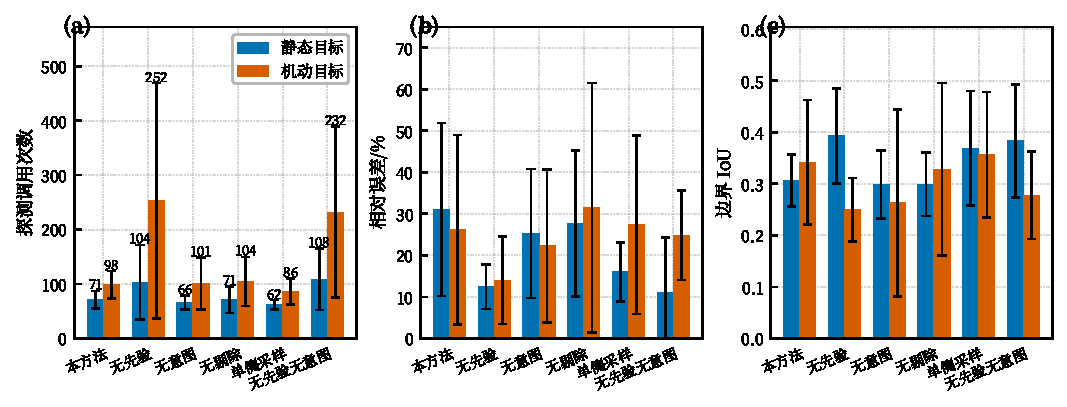
\includegraphics[width=0.72\textwidth]{fig_ablation.pdf}
  \caption{消融实验：探测次数、相对误差与边界 IoU 对比（柱为中位数，误差棒为中位绝对偏差）}
  \label{fig:ablation}
\end{figure*}

\begin{table*}[!t]
  \centering
  \caption{各配置十次重复的完整统计（未收敛指达到迭代上限 160 轮仍未满足 $\varepsilon$ 判据的重复次数；基线方法不适用该判据）}
  \label{tab:stats}
  \resizebox{\textwidth}{!}{%
  \begin{tabular}{lcccccc}
    \toprule
    方法 & 中位数[$Q_1,Q_3$] & 均值$\pm$标准差 & 最小--最大 & 未收敛 & 相对误差均值/\% & 边界 IoU \\
    \midrule
    \multicolumn{7}{l}{\sffamily 静态目标}\\
    \midrule
    本方法 & 71 [61, 87] & 80$\pm$28 & 54--144 & 0 & 31.2 & 0.333$\pm$0.070\\
    无先验 & 104 [66, 160] & 120$\pm$64 & 51--247 & 0 & 19.4 & 0.400$\pm$0.088\\
    无意图 & 66 [60, 76] & 74$\pm$29 & 51--150 & 0 & 27.2 & 0.298$\pm$0.072\\
    无剔除 & 71 [56, 85] & 76$\pm$30 & 51--152 & 0 & 30.9 & 0.322$\pm$0.075\\
    单侧采样 & 62 [57, 74] & 76$\pm$43 & 51--196 & 0 & 16.8 & 0.366$\pm$0.083\\
    无先验无意图 & 108 [68, 140] & 119$\pm$64 & 54--264 & 0 & 19.8 & 0.399$\pm$0.097\\
    信息增益 & 102 [89, 132] & 111$\pm$26 & 84--159 & 0 & 12.1 & 0.857$\pm$0.155\\
    全覆盖扫描 & 10000 [10000, 10000] & 10000$\pm$0 & 10000--10000 & -- & 2.1 & --\\
    随机采样 & 12500 [12000, 13750] & 12900$\pm$1449 & 11000--16000 & -- & 1.8 & --\\
    \midrule
    \multicolumn{7}{l}{\sffamily 机动目标}\\
    \midrule
    本方法 & 98 [72, 106] & 106$\pm$58 & 60--264 & 0 & 33.6 & 0.321$\pm$0.121\\
    无先验 & 252 [142, 394] & 316$\pm$271 & 54--980 & 0 & 33.2 & 0.235$\pm$0.095\\
    无意图 & 101 [68, 112] & 97$\pm$33 & 57--154 & 0 & 32.1 & 0.270$\pm$0.141\\
    无剔除 & 104 [73, 127] & 134$\pm$108 & 63--424 & 0 & 35.1 & 0.300$\pm$0.133\\
    单侧采样 & 86 [76, 112] & 95$\pm$27 & 64--150 & 0 & 34.2 & 0.327$\pm$0.120\\
    无先验无意图 & 232 [98, 320] & 244$\pm$183 & 54--661 & 0 & 24.4 & 0.233$\pm$0.097\\
    信息增益 & 220 [195, 360] & 262$\pm$109 & 144--423 & 0 & 16.7 & 0.353$\pm$0.061\\
    全覆盖扫描 & 10000 [10000, 10000] & 10000$\pm$0 & 10000--10000 & -- & 5.9 & --\\
    随机采样 & 13500 [13000, 14750] & 13500$\pm$2273 & 10000--17000 & -- & 2.1 & --\\
    \bottomrule
  \end{tabular}}%
\end{table*}

\subsection{参数敏感性与鲁棒性分析}

本节考察方法对关键超参数与输入质量的稳健性。为隔离被扫因素的影响，本小节各算例中策略参数固定为 LLM 编译值（不触发闭环重编译）。

（1）证据老化权重阈值 $\Delta$ 的敏感性。机动算例下扫描 $\Delta\in\{0.05,\ldots,0.80\}$（每取值 10 次重复，含超出合法值域 $[0.02,0.30]$ 的取值以考察边界行为），结果如图\ref{fig:delta}所示：探测次数中位数在整个扫描区间内持平于 80--84 次、边界 IoU 稳定于 0.24--0.26，表明收敛成本与判定精度对 $\Delta$ 取值不敏感。图\ref{fig:delta}(b)进一步给出机制层面的解释：老化机制的实际激活程度（复验单元格数）随 $\Delta$ 单调上升，$\Delta\leq0.15$ 时几乎不触发——典型收敛周期（约 25 轮迭代）内负样本权重尚来不及衰减到小阈值以下；$\Delta\geq0.45$ 后复验显著增加，个别重复因复验开销探测次数升至 180 次左右，但成本仍有界（中位数不变），亦有重复因及时复验过期命中而提前收敛。即机制真实起作用而成本保持有界，默认值 0.10 处于复验负荷与新鲜度之间的合理区间。

\begin{figure}[!t]
  \centering
  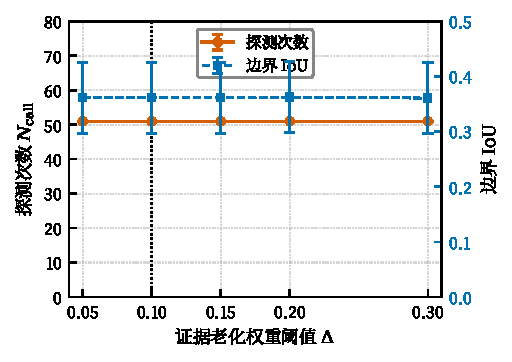
\includegraphics[width=\columnwidth]{fig_delta_sensitivity.pdf}
  \caption{机动算例下 $\Delta$ 阈值敏感性。（a）探测次数（中位数 $\pm$ 中位绝对偏差，散点为 10 次重复原始值）与边界 IoU；（b）复验单元格数均值——老化机制激活度随 $\Delta$ 上升而探测成本保持有界}
  \label{fig:delta}
\end{figure}

（2）先验质量鲁棒性。第 2.1 节声明“错误先验不改变收敛成本的最坏情形有界性”，此处予以实验验证：对 LLM 编译所得先验分别施加热点偏移（$0.1$/$0.2$/$0.3$ 归一化距离）、掺入虚假热点与全域错报先验，静态算例下各配置探测次数如图\ref{fig:prior}所示。全部失真先验的探测次数中位数均未超过无先验基线——失真先验不会拖慢收敛，成本有界性成立。同时须如实说明：先验质量仍影响判定精度，全域错报配置的平均边界 IoU 明显低于正确先验，表明精度收益以情报基本有效为前提，工程应用中需辅以情报可信度门控与多源校验。

\begin{figure}[!t]
  \centering
  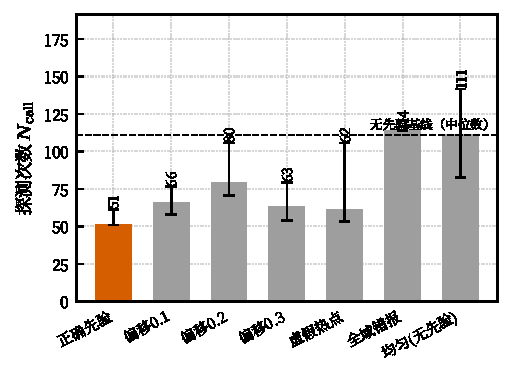
\includegraphics[width=\columnwidth]{fig_prior_robustness.pdf}
  \caption{静态算例下先验质量鲁棒性（柱为 10 次重复中位数，误差棒为中位绝对偏差；虚线为无先验基线中位数）}
  \label{fig:prior}
\end{figure}

（3）海域规模标度。将候选网格由 $40\times40$ 扩展至 $120\times120$，对比本方法与全覆盖扫描的探测次数随候选点数 $N$ 的增长趋势（对数坐标），如图\ref{fig:scale}所示。全覆盖扫描的探测次数随 $N$ 线性增长；本方法的增长显著低于线性，$N=14400$ 时探测成本仅为全覆盖的个位数百分比。值得注意的是，全覆盖扫描在 $N=14400$ 处因统一的 $\varepsilon$ 停机规则提前终止并给出错误估计（相对误差达 100\%）——在相同完备度判据下，边界主动采样的判定可靠性同样占优。

\begin{figure}[!t]
  \centering
  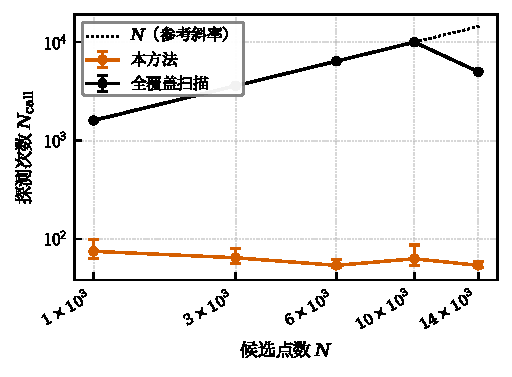
\includegraphics[width=\columnwidth]{fig_scale.pdf}
  \caption{探测次数随候选点数 $N$ 的增长趋势（对数坐标，10 次重复中位数，误差棒为中位绝对偏差；全覆盖扫描为确定性成本，逐次无随机波动，故无误差棒）}
  \label{fig:scale}
\end{figure}

（4）LLM 编译可靠性统计。对 8 类不同表述的情报文本与 8 类不同意图文本分别独立编译 5 次（共 80 次真实调用）：情报编译返回热点数 $2.7\pm0.8$ 个、先验置信度均值 $0.66$；意图编译参数统计见表\ref{tab:llm}。全部调用均返回合法结构化输出，未发生一次钳制触发——LLM 自发将参数约束在稳定域内，编译结果随文本表述的变化适度响应而不失控，说明语义编译机制在真实调用下稳定可用。

（5）观测噪声敏感性。将单次探测的漏警与虚警合并为概率 $p_f$ 的符号级误检（每次观测以 $p_f$ 概率返回符号翻转的证据值），静态算例下扫描 $p_f\in\{0,0.05,0.10\}$（各 10 次重复）：探测次数中位数由 $p_f=0$ 的 110 次增至 172/330 次，相对误差中位数由 26\% 升至 78\%/246\%，边界 IoU 均值由 0.40 降至 0.20/0.10。结果表明符号级误检显著拖累收敛成本与判定精度——方法依赖探测标签的基本正确性，对高误检传感器的稳健性有限，工程应用中需以多源观测投票或置信度加权缓解；该敏感性亦划定了第 3.1 节理想探测模型下本文结论的适用边界。

\begin{table}[!t]
  \centering
  \caption{LLM 意图编译参数统计（40 次真实调用）}
  \label{tab:llm}
  \resizebox{\columnwidth}{!}{% auto-generated by make_sweep_figures.py
\begin{tabular}{lccc}
\toprule
参数 & 均值$\pm$标准差 & 钳制触发率/\% & 取值界 \\
\midrule
$p_0$ & 0.54$\pm$0.13 & 0 & $[0.2,0.8]$ \\
$p_{\min}$ & 0.10$\pm$0.05 & 0 & $[0.02,0.30]$ \\
$\eta$ & 0.76$\pm$0.09 & 0 & $[0.60,0.95]$ \\
$\Delta$ & 0.10$\pm$0.06 & 0 & $[0.02,0.30]$ \\
$r_d$ & 0.53$\pm$0.10 & 0 & $[0.30,0.70]$ \\
$w_e$ & 1.11$\pm$0.17 & 0 & $[0.50,1.50]$ \\
$B$ & 4.15$\pm$1.25 & 0 & $[2,8]$ \\
\bottomrule
\end{tabular}}
\end{table}

\subsection{系统演示}

在搭建的仿真系统中对完整任务流程进行演示：系统接收文本情报与指挥意图后自动完成编译，多 UUV沿置信边界执行确认/排除任务，界面实时展示信念图演化、UUV 轨迹与每次任务重规划的自然语言理由。$\hat P_s$ 收敛至 $\pestS$ 且 $\varepsilon\leq0.02$ 后系统输出“目标不在该海域”的完备度声明，全过程探测成本仅为全覆盖方案的 $\ratio$\%。

% ============ 5 结论 ============
\section{结论与未来工作}

提出 LLM 语义编译主动学习搜索方法并搭建多 UUV 对海搜索仿真系统，主要结论如下：

（1）将结构可靠性 AL-DNN 框架迁移至对海搜索，以置信边界双侧主动采样替代几何覆盖，静态算例中以 $\callS$ 次探测达到全覆盖扫描 $\callL$ 次探测的同等判定置信度，探测成本降低 $\gainS$\%；

（2）语义编译机制将文本情报与指挥意图合法化注入搜索回路：消融实验表明先验引导使机动算例探测次数中位数较无先验配置降低约 61\%，意图闭环编译的成本效应不显著但提供了可审计的随态势调节能力，证据老化保障了漂移场景下边界跟踪的时效性；敏感性与鲁棒性实验进一步表明方法对老化阈值不敏感、失真先验下收敛成本仍有界、探测成本随海域规模呈亚线性增长，80 次真实 LLM 编译调用输出全部合法；

（3）LLM 仅输出有界参数与概率图、由确定性算法完成探测决策的分工模式，在引入语义能力的同时保持了方法的可审计性与收敛成本的最坏情形有界性。

本文仿真采用理想化探测与机动模型，真实声呐探测概率、海流扰动与多目标场景有待进一步验证；未来工作包括引入更真实的探测物理模型、异构传感器融合以及更大规模的UUV 集群协同搜索。

% ============ 参考文献 ============
\begin{thebibliography}{30}
\zihao{-5}
\setlength{\itemsep}{0pt}

\bibitem{ref1} 徐芑南, 吴有生. 潜水器设计[M]. 上海: 上海交通大学出版社, 2007. (Xu Q N, Wu Y S. Submersible design[M]. Shanghai: Shanghai Jiao Tong University Press, 2007.)
\bibitem{ref2} 陈延康, 朱文蔚. 无人潜航器技术发展现状与趋势[J]. 舰船科学技术, 2020, 42(7): 1-6. (Chen Y K, Zhu W W. Development status and trends of uncrewed underwater vehicle technology[J]. Ship Science and Technology, 2020, 42(7): 1-6.)
\bibitem{ref3} Choset H. Coverage for robotics---a survey of recent results[J]. Annals of Mathematics and Artificial Intelligence, 2001, 31(1): 113-126.
\bibitem{ref4} Galceran E, Carreras M. A survey on coverage path planning for robotics[J]. Robotics and Autonomous Systems, 2013, 61(12): 1258-1276.
\bibitem{ref5} Bourgault F, Furukawa T, Durrant-Whyte H F. Optimal search for a lost target in a Bayesian world[C]//Field and Service Robotics. Berlin: Springer, 2003: 209-222.
\bibitem{ref6} Lanillos P, Besada-Portas E, Pajares G, et al. Minimum time search for lost targets using cross entropy optimization[C]//IEEE/RSJ International Conference on Intelligent Robots and Systems. IEEE, 2012: 602-609.
\bibitem{ref7} Hu S, Ni W. Reinforcement learning-based search algorithm for autonomous underwater vehicles[J]. IEEE Access, 2020, 8: 165423-165432.
\bibitem{ref8} Cao Z, Li B, Wang X, et al. Target search with UAV swarm based on deep reinforcement learning[J]. IEEE Transactions on Vehicular Technology, 2022, 71(9): 9873-9884.
\bibitem{ref9} 翟东升, 周晓红, 周立成, 等. 基于主动学习深度神经网络模型的结构可靠性分析方法[J]. 应用力学学报, 2024, 41(5): 1092-1101. (Zhai D S, Zhou X H, Zhou L C, et al. Structural reliability analysis method based on active learning deep neural network model[J]. Chinese Journal of Applied Mechanics, 2024, 41(5): 1092-1101.)
\bibitem{ref10} Brown T B, Mann B, Ryder N, et al. Language models are few-shot learners[C]//Advances in Neural Information Processing Systems. 2020: 1877-1901.
\bibitem{ref11} Zhao W X, Zhou K, Li J, et al. A survey of large language models[J]. arXiv preprint arXiv:2303.18223, 2023.
\bibitem{ref12} Ahn M, Brohan A, Brown N, et al. Do as I can, not as I say: grounding language in robotic affordances[C]//Conference on Robot Learning. PMLR, 2022: 287-318.
\bibitem{ref13} Huang W, Xia F, Xiao T, et al. Inner monologue: embodied reasoning through planning with language models[C]//Conference on Robot Learning. PMLR, 2023: 1769-1782.
\bibitem{ref14} Echard B, Gayton N, Lemaire M. AK-MCS: an active learning reliability method combining Kriging and Monte Carlo simulation[J]. Structural Safety, 2011, 33(2): 145-154.
\bibitem{ref15} Xiang Z, Chen J, Bao Y, et al. An active learning method combining deep neural network and weighted sampling for structural reliability analysis[J]. Mechanical Systems and Signal Processing, 2020, 140: 106684.
\bibitem{ref16} Li J, Wang D. Structural reliability analysis based on ensemble learning and active learning[J]. Reliability Engineering \& System Safety, 2022, 217: 108134.
\bibitem{ref17} Karpatne A, Kannan R, Kumar V. Knowledge guided machine learning: accelerating discovery using scientific knowledge and data[M]. Boca Raton: CRC Press, 2022.
\bibitem{ref18} Stone L D. Theory of Optimal Search[M]. New York: Academic Press, 1975.
\bibitem{ref19} 姚尧, 潘光, 李霄, 等. 多无人潜航器协同搜索技术研究综述[J]. 水下无人系统学报, 2021, 29(4): 369-379. (Yao Y, Pan G, Li X, et al. A survey on cooperative search technology of multiple UUVs[J]. Journal of Unmanned Undersea Systems, 2021, 29(4): 369-379.)
\bibitem{ref20} 朱大奇, 刘菲. 多自主水下航行器协同控制技术研究综述[J]. 控制与决策, 2019, 34(10): 2017-2026. (Zhu D Q, Liu F. A survey on cooperative control technology of multiple autonomous underwater vehicles[J]. Control and Decision, 2019, 34(10): 2017-2026.)
\bibitem{ref21} Sharon G, Stern R, Felner A, et al. Conflict-based search for optimal multi-agent pathfinding[J]. Artificial Intelligence, 2015, 219: 40-66.
\bibitem{ref22} Dubins L E. On curves of minimal length with a constraint on average curvature, and with prescribed initial and terminal positions and tangents[J]. American Journal of Mathematics, 1957, 79(3): 497-516.
\bibitem{ref23} Wang X, Yao L, Wang Z, et al. Sea mine search strategy for AUV swarm based on information gain[J]. Ocean Engineering, 2021, 237: 109563.
\bibitem{ref24} Krishna A, Sridharan M. Agentic large language models for autonomous systems: a survey[J]. ACM Computing Surveys, 2024, 56(9): 1-38.

\end{thebibliography}

\vspace{12pt}
\begin{center}
  {\zihao{-2}\bfseries Active-Learning Multi-UUV Sea-Target Search Empowered by LLM Semantic Compilation\par}
  \vspace{8pt}
  {\zihao{-4} Author One$^{1}$, Author Two$^{1}$, Author Three$^{2}$\par}
  \vspace{4pt}
  {\zihao{-5} (1. XX University, XX 000000, China; 2. XX Institute, XX 000000, China)\par}
\end{center}
{\zihao{-5}\sffamily\bfseries Abstract: }{\zihao{-5}
To address the low efficiency of lawnmower coverage and the difficulty of injecting textual intelligence and commander intent into numerical search loops in multi-UUV sea-target search, this paper proposes an active-learning search method empowered by large language model (LLM) semantic compilation. The sea area is discretized into candidate probing points; a deep neural network maintains an online target-presence belief map and approximates the confidence boundary, along which confirm and exclude probing tasks are generated on both sides. The LLM acts as a semantic compiler: intelligence reports are compiled into a target-presence prior for guided initial sampling, while commander intent and real-time situation are compiled into bounded acquisition parameters, achieving legitimate injection of language information into numerical control. A multi-UUV search simulation system integrating belief inference, task allocation and multi-vehicle path planning is built. Experiments on a $10^4$-cell area show that the proposed method reaches the same decision confidence as full-coverage search with a median of $\callS$ probing calls versus 10\,000 ($\ratio$\% of its cost, $\gainS$\% lower); ablation verifies the contribution of each semantic-compilation component.
\par}
\vspace{4pt}
{\zihao{-5}\sffamily\bfseries Key words: }{\zihao{-5} sea-target search; active learning; large language model; deep neural network surrogate; multi-UUV\par}

\end{document}
